\documentclass{beamer}
%\title{text}
%\author{text}
%\date{date}
\usetheme{Boadilla}

\usepackage{tikz}
\usetikzlibrary{mindmap,trees}
\usepackage{verbatim}
\usepackage{adjustbox}
\usepackage[utf8]{inputenc} % diacritice

\begin{document}

\begin{frame}{MINDMAP}
\resizebox{\textwidth}{!}{
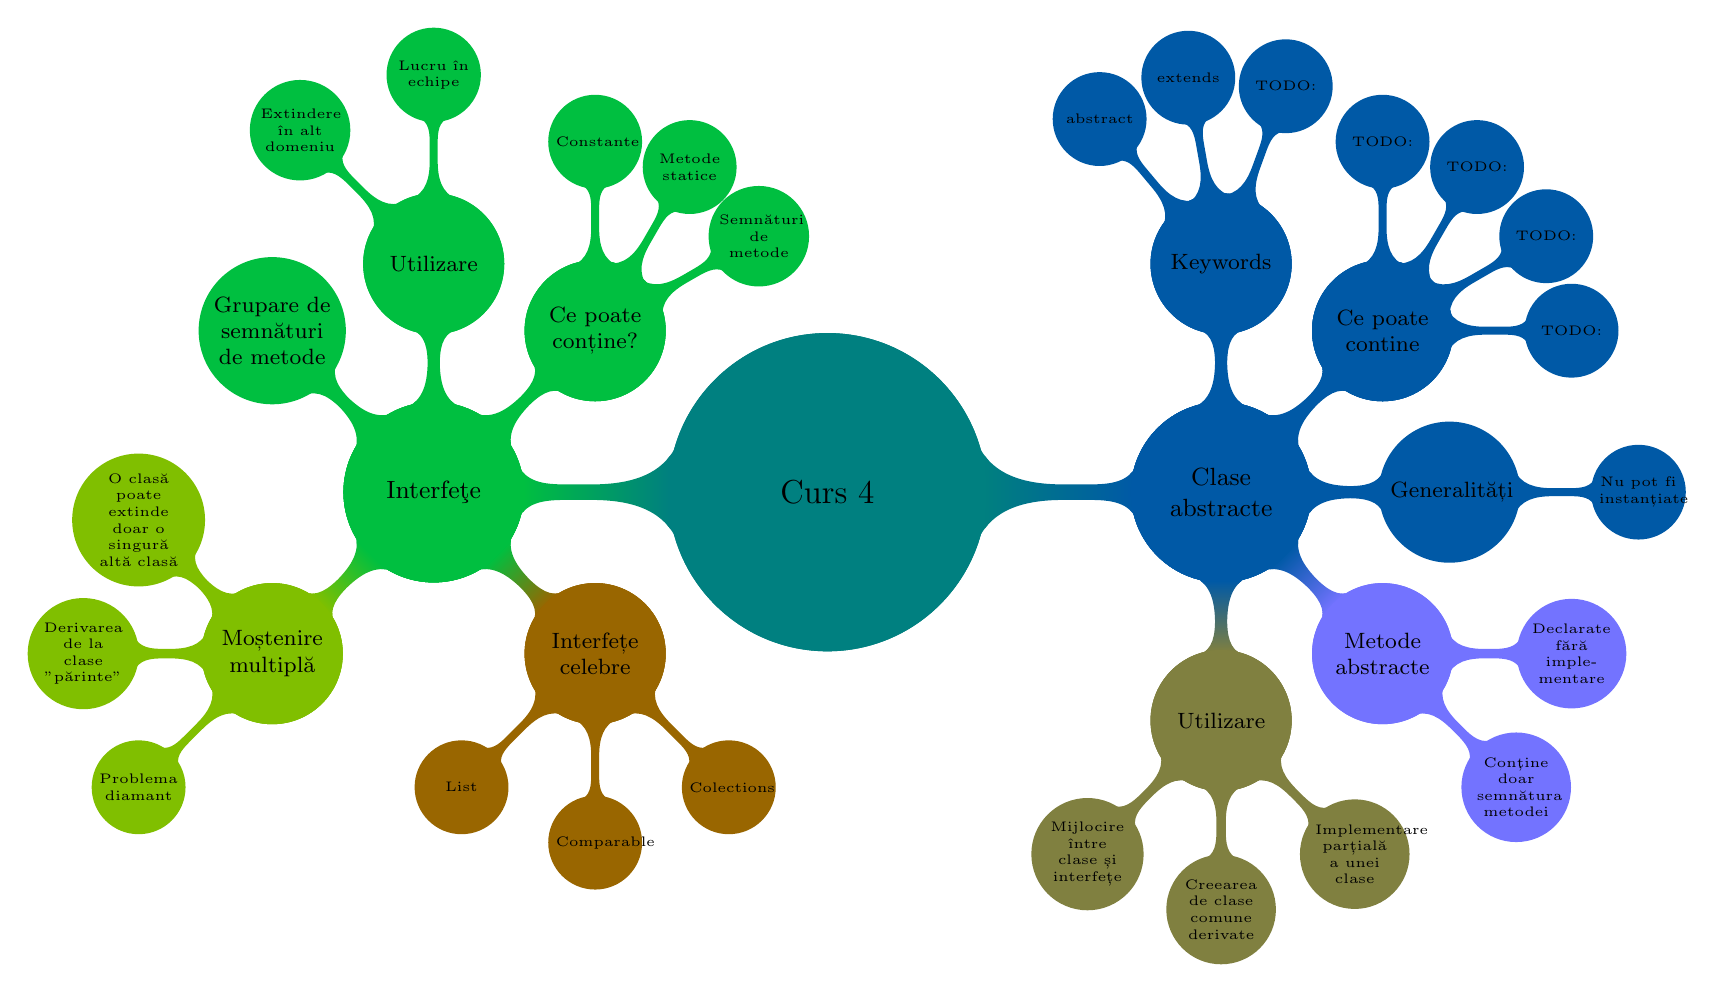
\begin{tikzpicture}
 	\path[mindmap, concept color=teal,text=black]
	node[concept] {Curs 4} [clockwise from=0]
	child[concept color = blue!30!teal] {
		node[concept] {Clase abstracte} [clockwise from=-45]
			child[concept color = white!45!blue]{
				node[concept] {Metode abstracte}[clockwise from=0] {child{node[concept]{Declarate fără implementare}}}
				node[concept] {Metode abstracte}[clockwise from=-45] {child{node[concept]{Conține doar semnătura metodei}}}
}
		node[concept] {Clase abstracte} [clockwise from=90]
			child[concept color = blue!30!teal] {
			node[concept] {Keywords}[clockwise from=130] {child{node[concept]{abstract}}}
			node[concept] {Keywords}[clockwise from=100] {child{node[concept]{extends}}}
			node[concept] {Keywords}[clockwise from=70] {child{node[concept]{TODO:}}}
}		
		node[concept] {Clase abstracte} [clockwise from=45]
			child[concept color = blue!30!teal] {
			node[concept] {Ce poate contine}[clockwise from=90] {child{node[concept]{TODO:}}}
			node[concept] {Ce poate contine}[clockwise from=60] {child{node[concept]{TODO:}}}
			node[concept] {Ce poate contine}[clockwise from=30] {child{node[concept]{TODO:}}}
			node[concept] {Ce poate contine}[clockwise from=0] {child{node[concept]{TODO:}}}
}
		node[concept] {Clase abstracte} [clockwise from=0]
			child[concept color = blue!30!teal]{
			node[concept] {Generalități}[clockwise from = 0] {child{node[concept]{Nu pot fi instanțiate}}}
}
		node[concept] {Clase abstracte} [clockwise from=-90]
			child[concept color = orange!50!teal]{
				node[concept]{Utilizare}[clockwise from = -90] {child{node[concept]{Creearea de clase comune derivate}}}
				node[concept]{Utilizare}[clockwise from = -45] {child{node[concept]{Implementare parțială a unei clase}}}
				node[concept]{Utilizare}[clockwise from = -135] {child{node[concept]{Mijlocire între clase și interfețe}}}
}
}
	node[concept] {Curs 4} [clockwise from=180]
	child[concept color = green!50!teal] {
		node[concept] {Interfețe} [clockwise from=45]
			child[concept color = green!50!teal]{
				node[concept]{Ce poate conține?}[clockwise from = 30]{child{node[concept]{Semnături de metode}}}
				node[concept]{Ce poate conține?}[clockwise from = 60]{child{node[concept]{Metode statice}}}
				node[concept]{Ce poate conține?}[clockwise from = 90]{child{node[concept]{Constante}}}
}
		node[concept] {Interfețe} [clockwise from=135]
			child{node[concept] {Grupare de semnături de metode} }
		node[concept] {Interfețe} [clockwise from=90]
			child[concept color = green!50!teal]{
				node[concept] {Utilizare} [clockwise from = 90] {child{node[concept]{Lucru în echipe}}}
				node[concept] {Utilizare} [clockwise from = 135] {child{node[concept]{Extindere în alt domeniu}}}
}
		node[concept] {Interfețe} [clockwise from=-45]
			child[concept color = red!60!green]{
					node[concept] {Interfețe celebre} [clockwise from = 225] {child{node[concept]{List}}}
					node[concept] {Interfețe celebre} [clockwise from = -90] {child{node[concept]{Comparable}}}
					node[concept] {Interfețe celebre} [clockwise from = -45] {child{node[concept]{Colections}}}
}
		node[concept] {Interfe\c te} [clockwise from=225]
			child[concept color = orange!50!green]{
				node[concept] {Moștenire multiplă} [clockwise from=180] {child{node[concept]{Derivarea de la clase "părinte"}}}
				node[concept] {Moștenire multiplă} [clockwise from=135] {child{node[concept]{O clasă poate extinde doar o singură altă clasă}}}
				node[concept] {Moștenire multiplă} [clockwise from=225] {child{node[concept]{Problema diamant}}}
}
}
;
\end{tikzpicture}
}
\end{frame}
\end{document}
